%\documentclass[3p,preprint]{elsarticle}
\documentclass[3p,twocolumn]{elsarticle}
\usepackage{lineno,hyperref}
\usepackage{amsmath}
\usepackage{ifthen}
\usepackage{commath}
\usepackage{amssymb}
\usepackage{scalerel}
\usepackage{natbib}

\usepackage{adjustbox}   
\usepackage{threeparttable}
\usepackage{booktabs}
\usepackage{colortbl} 
\usepackage{xcolor}
\usepackage{float}
\usepackage{flafter}

\newcommand{\diff}[2]{\dfrac{\partial #1}{\partial #2}}

\usepackage{amssymb}
\usepackage{amsmath}
\usepackage{commath}
\usepackage{graphicx,bm}
\usepackage[]{subfig}
\usepackage{epstopdf}

\biboptions{sort&compress}
\modulolinenumbers[5]

\journal{Journal of \LaTeX\ Templates}

%%%%%%%%%%%%%%%%%%%%%%%
%% Elsevier bibliography styles
%%%%%%%%%%%%%%%%%%%%%%%
%% To change the style, put a % in front of the second line of the current style and
%% remove the % from the second line of the style you would like to use.
%%%%%%%%%%%%%%%%%%%%%%%
%% Numbered
%\bibliographystyle{model1-num-names}

%% Numbered without titles
\bibliographystyle{model1a-num-names}

%% Harvard
%\bibliographystyle{model2-names.bst}\biboptions{authoryear}

%% Vancouver numbered
%\usepackage{numcompress}\bibliographystyle{model3-num-names}

%% Vancouver name/year
%\usepackage{numcompress}\bibliographystyle{model4-names}\biboptions{authoryear}

%% APA style
%\bibliographystyle{model5-names}\biboptions{authoryear}

%% AMA style
%\usepackage{numcompress}\bibliographystyle{model6-num-names}

%% `Elsevier LaTeX' style
%\bibliographystyle{elsarticle-num}
%%%%%%%%%%%%%%%%%%%%%%%

\begin{document}

\begin{frontmatter}

\title{A molecular dynamics study of the solvation of CO\textsubscript{2}, water, and some organic compounds in the ionic liquids [emim][B(CN)\textsubscript{4}] and [emim][NTf\textsubscript{2}]}

%% Group authors per affiliation:
\author[rvt]{A.J.~Silveira}
\author[rvt]{S.~Pereda}
\author[focal,els]{F.W.~Tavares}
\author[focal]{C.R.A.~Abreu\corref{cor1}}
\ead{abreu@eq.ufrj.br}

\address[rvt]{Planta Piloto de Ingenier\'ia Qu\'imica, PLAPIQUI, Universidad Nacional del Sur,Camino La Carrindanga Km 7-CC: 717, Bah\'ia Blanca, Argentina}
\address[focal]{Chemical Engineering Department, Escola de Qu\'imica, Universidade Federal do Rio de Janeiro,Rio de Janeiro, RJ 21941-909, Brazil}
\address[els]{COPPE, Universidade Federal do Rio de Janeiro, Rio de Janeiro, RJ 21941-909, Brazil}

\cortext[cor1]{Corresponding author}

\begin{abstract}
In this paper we predict solvation in ionic liquids and macroscopic properties required in the design of chemical processes. Carbon dioxide produced in combustion processes is one of the main sources of anthropogenic generation of greenhouse gases. On the other hand, the potential of [emim][B(CN)\textsubscript{4}] for its capture has recently been reported. For comparison, the solvents [emim][B(CN)\textsubscript{4}] and [emim][Tf\textsubscript{2}N] were analyzed, both in the condition of infinite dilution and at high concentrations. The simulations confirmed what was observed experimentally, that is, a considerably lower pressure is required in [emim][B(CN)\textsubscript{4}] to obtain the same molality of CO\textsubscript{2}. The infinite-dilution activity coefficients of solutes hexane, benzene, cyclohexane, ethanol, and water in [emim][B(CN)\textsubscript{4}] were also calculated, and a comparison was made with experimental values recently reported in the literature.
\end{abstract}

\begin{keyword}
ionic liquids \sep solvation free energy \sep  CO\textsubscript{2} 
\end{keyword}

\end{frontmatter}

\linenumbers

\section{Introduction}
State the objectives of the work and provide an adequate background, avoiding a detailed literature survey or a summary of the results.

The CO\textsubscript{2} emissions from power generation plants are still sources of anthropogenic greenhouse gases~\cite{totalenergy} and the searching of solvents is an active field of research. Post combustion absorption technologies flue gas

Basically, the conventional process for CO\textsubscript{2} removal involves a chemical absorption followed by stripping at high temperatures. The solvents commonly used are volatile organic compounds, specially aqueous solutions of monoethanolamine (MEA). Despite its high absorption capability, the use of MEA suffers from a serious drawback in that there is considerable cost due to the energy consumption in the solvent recovery~\cite{Merkel_2010}. Other disadvantages include corrosion and degradation by oxidation, solvent loss by evaporation, which also contributes with ambient pollution and generates extra costs for substituting the solvent.

The investigation of ionic liquids (ILs) as alternative solvents for CO\textsubscript{2} sequestration occupies a central place. The reasons in their well known properties, such as the negligible vapor pressure and high thermal stability. Furthermore, they are particularly attractive because they can be designed for specific applications, giving rise to the so-called task-specific ionic liquids~\cite{Seo_2014}. These remarkable properties makes ionic liquids suitable for a wide variety of applications in separation processes~\cite{Han_2010,Werner_2010}, catalysis~\cite{P_rvulescu_2007}, energy~\cite{MacFarlane_2014} and material science~\cite{Mecerreyes_2011,Tom_2015,Dupont_2010,Leones_2017,Kinik_2017}.

Recently, the potentiality of ionic liquids for CO\textsubscript{2} capture has been called into question by Carvalho~\textit{et al.}~\cite{Carvalho_2016}, who warn that the use of molar fraction to express solubility has, to some extent, perpetuated misconceptions regarding the supposed absorption capability of certain ionic liquids. While most thermodynamic models are developed based on molar fraction, the key factor to determine the absorption process efficiency is given by the amount of CO\textsubscript{2} that can be dissolved in a certain volume or mass of solvent. By expressing the solubility in terms of molality and performing an exhaustive comparison between various ionic liquids, Ref.~\cite{Carvalho_2016} shows that most systems which promote a physical absorption of CO\textsubscript{2} exhibit a CO\textsubscript{2} solubility similar or even lower than that observed for the heavy alkane eicosane. This is true for the ``popular'' [bmim][Tf\textsubscript{2}N], [bmim][PF\textsubscript{6}], [bmim][BF\textsubscript{4}], as well as for those synthesized from the fluorination of the cation or the anion, such as [(C\textsubscript{2}H\textsubscript{2}F\textsubscript{2})mim][NTf\textsubscript{2}] and [hmim][pFAP], the only exception being the family of ionic liquids containing the anion tetracyanoborate [B(CN)\textsubscript{4}]$^{-}$.

There is no obvious explanation accounting for the enhanced solubility promoted by the presence of the anion [B(CN)\textsubscript{4}]$^{-}$, whether special interactions with CO\textsubscript{2} are settled. In this sense, Molecular Simulation provides with a powerful tool for studying solvation processes. To our knowledge, only one study in the literature reports the free energy of solvation of CO\textsubscript{2} in [emim][B(CN)\textsubscript{4}] which, in addition, is overestimated. This motivated us to carry out a comparison of different force fields of [emim][B(CN)\textsubscript{4}] in terms of the free energy of solvation and, indeed,  it was possible to select a model that successfully predicts the value of the Henry constant of CO\textsubscript{2}. For comparison, the solvents [emim][B(CN)\textsubscript{4}] and [emim][Tf\textsubscript{2}N] were analyzed, both in the condition of infinite dilution and at high concentrations. The simulations confirmed what was observed experimentally, that is, a considerably lower pressure is required in [emim][B(CN)\textsubscript{4}] to obtain the same molality of CO\textsubscript{2}. The infinite-dilution activity coefficients of solutes hexane, benzene, cyclohexane, ethanol, and water in [emim][B(CN)\textsubscript{4}] were also calculated, and a comparison was made with experimental values recently reported in the literature.

This paper is organized as follows: in Section~\ref{sec:theory} we present some methodological details, including the mathematical relationships between free energy of simulated solvation and thermodynamic properties of diluted solutions. and a brief description of the force fields considered for [emim][B(CN)\textsubscript{4}], and the details of the simulations for free energy calculations are presented. The corresponding results are presented in the Section~\ref{sec:results}, where a comparison is made with the experimental data of Henry's constants, the results of the activity coefficients are shown at infinite dilution and, finally, a study of the CO\textsubscript{2} solvation is carried out in high concentrations.

\section{Theoretical background}
\label{sec:theory}

In this section, we present the formalism that allows a direct comparison between simulation results and the thermodynamic properties of dilute solutions: Henry constant and activity coefficient at infinite dilution. For this, we rely on the work of Shirts~\textit{et al.}~\cite{Shirts_2003}. Then, we reformulate the equations in order to carry out a study at concentrated conditions, which would be the more likely scenario in CO\textsubscript{2} capture processes.

\subsection*{Solvation free energy}
The solvation free energy, $\Delta G_{\text{solv}}$, is the reversible work needed to transfer a solute molecule from the gas phase to the solution. For dense systems, an efficient computation of solvation properties via molecular simulation is possible by means of the so-called alchemical methods, which employ non-physical pathways to connect the ``endpoint'' states, whose free energy difference is to be estimated. In the case of $\Delta G_{\text{solv}}$, the alchemical route involves a gradual insertion/deletion of the solute through a coupling parameter $\lambda$, which scales the intermolecular interactions taking values in the interval [0,1]: $\lambda$ = 1 corresponds to a fully interacting system, while for $\lambda$ = 0 the interactions between the solute and solvent molecules are completely turned-off.

In the following, the subscripts ``$s$'' and ``$\text{IL}$'' refer to the solute and the solvent (ionic liquid), respectively. For a system containing $N_{\text{IL}}$ solvent molecules and $N_{\text{s}}$ solute molecules at fixed pressure (P) and temperature (T), the difference in free energy between the states associated to $\lambda$ = 1 and $\lambda$ = 0 is defined as
\begin{equation}
\Delta G_{\text{sim}} \equiv k_b T \ln \frac{\bigtriangleup (N_s^l,N_{LI},P,T,\lambda = 1)}{\bigtriangleup (N_s^l,N_{LI},P,T,\lambda = 0)}, 
\end{equation}
where $\bigtriangleup$ denotes the isobaric-isothermal partition function. Shirts~\textit{et al}.~\cite{Shirts_2003} presented a detailed mathematical derivation allowing to relate $\Delta G_{\text{sim}}$ to what is experimentally known as the solvation free energy and obtained the following expression: 
\begin{equation}
\begin{split}
\label{eq:free_solv}
 \Delta G_{\text{solv}}& =  k_b T \ln \left( \frac{P_s}{c_s^{\ast} k_b T} \right)\\ &= \Delta G_{\text{sim}} - k_bT \ln \left( \frac{V^{\ast}}{V_1} \right) ,
\end{split}
\end{equation}
where $k_b$ is the Boltzmann's constant, $V^{\ast}$ and $V_1$ refer to the mean volumes of the systems specified by ($N_s^l-1$,$N_{\text{LI}}$,P,T) and ($N_s^l$,$N_{\text{LI}}$,P,T), respectively; $c_s^{\ast}$ = $N_s^l/V_1$ is the numerical concentration of the solute in the liquid phase and $P_s$ is the partial pressure of the solute in the gas phase. It should be noted that in the derivation of Eq.~\ref{eq:free_solv}, the gas phase was treated as an ideal gas. 

For small solutes, such as those considered in this work, the magnitude of the term $V^{\ast}/V_1$ is typically on the order of the free energy uncertainties~\cite{Shirts_2003}. Hence, that term could be neglected and will be omitted hereafter.

\subsection*{Henry constant}
If both $P_s$ and $c_s^{\ast}$ were not large, we can employ Eq.~\ref{eq:free_solv} to predict Henry's law constant $\text{K}_s$, which is given by~\cite{Prausnitz}
\begin{equation}
\text{K}_s =\frac{P_s}{x_s}.
\end{equation}
Therefore, by simply expressing Eq.~\ref{eq:free_solv} in terms of the molar fraction $x_s$ and considering MW (molecular weight of the solution) = $\text{MW}_{\scaleto{LI}{4pt}}$ as well as $\rho$ (mass density of the solution) = $\rho_{\scaleto{LI}{4pt}}$, we obtain that
\begin{equation}
\label{eq:henry_eq}
K_s = \tilde{\rho}_{\scaleto{LI}{4pt}} R T \exp(\beta \, \Delta G_{\text{sim}}),
\end{equation}
where $R$ is the gas constant.

\subsection*{Infinite-dilution activity coefficient}

As will be shown below, the prediction of activity coefficients requires separate simulations in the pure solute, and in what follows we employ the superscript ``$0$'' to denote the pure solute properties.

Using standard thermodynamic relations~\cite{Tester}, we write the activity coefficient $\gamma_s$ in terms of residual chemical potentials, as follows
\begin{equation}
\label{eq:gamma}
\ln \gamma_s = \frac{1}{RT} (\mu_s^R - \mu_s^{R,0}),
\end{equation}
where $\mu_s^R$ and $\mu_s^{R,0}$ are the residual chemical potentials of the solute in the solution and in the pure solute, respectively. It is worth noting that we have used the definition $\mu_s^{R}$ (P,T) = $\mu_s$ (P,T) - $\mu_s^{ig}$ (P,T), where the superscript $ig$ refers to a solution of ideal gases. Also, recall that $\mu_s^{ig} (P,T)$ = $\mu_s^{ig,0} (P,T)$ + $RT \ln x_s$, so we have that
\begin{equation}
\mu_s^R = \mu_s^l(N_s^l,N_{LI},P,T) - \mu_s^{ig,0}(P,T) - k_b T \ln x_s. 
\end{equation}
Replacing $\mu_s^{l}$ and $\mu_s^{ig,0}$ by the corresponding expressions derived in Ref.~\cite{Shirts_2003} yields
\begin{equation}
\label{eq:mu_res}
\mu_s^R = \Delta G_{\text{sim}} - k_b T \ln \left( \frac{V^{\ast} P}{N_s^l k_b T} \right) -  k_b T \ln x_s.
\end{equation}
Of course, an analogous equation holds for $\mu_s^{R,0}$:
\begin{equation}
\label{eq:mu_res_0}
\mu_s^{R,0} = \Delta G_{\text{sim}}^{0} - k_b T \ln \left( \frac{V^{\ast,0} P}{N_s^{l,0} k_b T} \right).
\end{equation}

Considering $N_s^{l}$ = 1, which represents the infinite-dilute condition, and substituting Eqs.~\ref{eq:mu_res} and~\ref{eq:mu_res_0} into Eq.~\ref{eq:gamma}, we  obtain that
\begin{equation}
\ln \gamma^{\infty}_s = \frac{1}{k_b T} \left( \Delta G_{\text{sim}} - \Delta G_{\text{sim}}^{0} \right) + \frac{c_{\scaleto{LI}{4pt}}^{\, \ast}}{c_{\, s}^{\, \ast,0}},
\end{equation}
where $c_{\scaleto{LI}{4pt}}^{\, \ast}$ y $c_{\, s}^{\, \ast,0}$ correspond to the numerical densities of the solvent and the pure solute, respectively.

\subsection*{Partial pressure estimation}

For the ILs of interest to the present investigation, high concentrations of CO\textsubscript{2} are found at pressure values for which, in principle, the ideal gas assumption may be not valid. In this case, we shall correct the ideal gas contribution to the chemical potential, as follows
\begin{equation}
\label{eq:mu_gas_real}
\mu^{g}_s = \mu^{ig}_s + RT \ln \phi_s,
\end{equation}
where $\phi_s$ is the fugacity coefficient of the solute. This equation, together with the fact that $f^{g}_s$ = $P_s \phi_s$, are used to evaluate $\mu^{l}_s$ = $\mu^{g}_s$, which yields
\begin{equation}
\label{eq:fgas_d}
f^{g}_s = \exp  \left( \beta \Delta G_{\text{sim}} \right) +  k_b T c_s^{\ast}, 
\end{equation}
where $f^{g}_s$ is the fugacity of the solute in the gas phase. Having calculated $f^{g}_s$, $P_s$ could be predicted using the following equation
\begin{equation}
\label{eq:fgas}
f^{g}_s = P_s \exp\left[ \frac{B_s(T) P_s}{R T} \right],
\end{equation}
where $B_s$ corresponds to the second virial coefficient. Here we employ the correlation for CO\textsubscript{2} introduced by Holste~\textit{et al}~\cite{Holste_1987}, which is
\begin{equation}
B_s = B_0 + \frac{B_1}{T} + \frac{B_2}{T^2},
\end{equation}
where $B_0$ = 23.02991 cm$^3$/mol, $B_1$ = $-2.455297$ $\times$ 10$^3$ (Kcm$^3$/mol) and $B_2$ = -1.22675$\times$10$^7$ (K$^2$cm$^3$/mol). Actually, the prediction of $P_s$ should be iterative and in this work we propose the following scheme: (i) run an NPT simulation, (ii) calculate $\Delta G_{\text{sim}}$ and $f^{g}_s$ via Eq.~\ref{eq:fgas_d}, (iii) employ $f^{g}_s$ in Eq.~\ref{eq:fgas} to compute $P_s$ (iv) if $P_s$ $\neq$ P, repeat the above steps using $P_s$ as the specified pressure in a new NPT simulation. This is done until $P_s$ = P.

\section{Force fields}
\label{sec:force_field}
\subsection{Ionic liquids}
\label{sec:force_field_il}

The versatility of ILs for different applications is in part due to the fact that their physical properties strongly depend on the cation-anion combination. On the other hand, this characteristic also explains why the desirable transferability of force fields is particularly difficult to attain. Indeed, it is a common practice to extract the potential parameters corresponding to intramolecular (bond stretching, angle bending, torsion rotation) and Lennard-Jones interactions from a well established force field and then derive the partial atomic charges. This procedure is, however, inaccurate as in conventional force fields the determination of the atomic charges precedes the dihedrals parametrization. Another ad-hoc strategy, which intends to crudely incorporate polarization effects, is to scale the partial charges uniformly with a factor which normally takes values in the range 0.8-0.9. This practice has proven to be effective in improving the predictions of dynamic properties~\cite{Schr_der_2012}.

In this paper, we consider four models of [emim][B(CN)\textsubscript{4}]. Koller~\textit{et al.}~\cite{Koller_2012} were the first to introduce a specific non-polarizable force field of [emim][B(CN)\textsubscript{4}]. They tested three variations of a \textit{united-atoms} model, in which the alkyl groups $\text{CH}_3$ y $\text{CH}_2$ of [emim]$^{+}$ are replaced by pseudo-atoms. Among them, the ``FF-3'' model best reproduces the experimental values of density, self-diffusion coefficients and viscosity. In short, both the intramolecular and Lennard-Jones parameters of the cation were taken from the work of Liu~\textit{et al.}~\cite{Liu_2006}, which in turn is based on the AMBER~\cite{Cornell_1995} framework. The intramolecular parameters involving the boron atom were extracted from the DREIDING~\cite{Mayo_1990} force field and the anionic vdW parameters were refined based on the values reported by Price~\textit{et al.}~\cite{Price_2001}. The atomic partial charges were derived using the EA-RESP method~\cite{Basma_2001} from \textit{Post-Hartree-Fock ab-initio} calculations at MP2/6–31G$^\ast$+ level of theory, which automatically resulted in total charges on the ions of $\pm$0.8426e. 

The potential parameters of [B(CN)\textsubscript{4}]$^{-}$ derived by Koller~\textit{et al.}~\cite{Koller_2012} were employed by Batista~\textit{et al.}~\cite{Batista_2015} to study aqueous solutions of [emim][B(CN)\textsubscript{4}]. In this case,  the authors considered the \textit{all-atom} model of [emim]$^{+}$ developed by Cadena and Maginn~\cite{Cadena_2006}. The atomic partial charges were obtained using the CHELP procedure~\cite{Breneman_1990}, resulting in net charges of $\pm$0.889$e$ on the ions. It should be noted that those force fields consider different scaling factors for 1-4 non-bonded interactions: Cadena and Maginn~\cite{Cadena_2006} use values of 1.0 y 0.4 for the Lennard-Jones and Coulombic interactions, respectively, while in Koller~\textit{et al.}~\cite{Koller_2012} the corresponding factors are 0.5 y 5/6, in accordance with AMBER force field. Batista~\textit{et al.}~\cite{Batista_2015} employ the same factors as Cadena and Maginn~\cite{Cadena_2006} (J.P. Coutinho, personal communication).

Another set of parameters for [emim][B(CN)\textsubscript{4}] was derived by Liu \textit{et al.}.~\cite{Liu_2014} in a study that investigates the dynamics of CO\textsubscript{2} and N\textsubscript{2} in that IL. Parameters corresponding to the intramolecular and Lennard-Jones interactions were extracted from GAFF~\cite{Wang_2004}, while the atomic partial charges were computed using the RESP method~\cite{Bayly_1993} from \textit{DFT}/B3LYP/6-311+G(d) calculations. The net charges of the ions were manually adjusted to a value of $\pm$0.8$e$.

We also consider the parametrization recently reported by Weber and Kirchner~\cite{Weber_2016}, which is based on the force field developed by P{\'{a}}dua and Canongia Lopes~\cite{Canongia_Lopes_2006}. The potential parameters for the anion are not specified in Refs.~\citenum{Weber_2016} and~\citenum{Canongia_Lopes_2006}, and we obtained them by a direct communication with the authors of Ref.~\citenum{Weber_2016}. The atomic partial charges were derived using the RESP procedure from \textit{Hartree-Fock} calculations at 6-31++G$^{\ast \ast}$ level of theory, resulting in net charges of $\pm$0.8$e$.

Finally, for [emim][Tf\textsubscript{2}N] we use the model of K\"{o}ddermann~\textit{et al}~\cite{K_ddermann_2007}, which result from ``refining'' the force field due to P{\'{a}}dua and Canongia Lopes~\cite{Canongia_Lopes_2006}. This ``refining'' was characterized by their authors as unusual, given that the LJ parameters were modified, while keeping the partial charges at their original values. This model was recently employed by Kerl~\textit{et al.}~\cite{Kerl__2017}, who were able to accurately predict Henry's constant for CO\textsubscript{2} at several temperatures.

\subsection{Solutes}
\label{sec:force_field_sol}

The solutes considered here are hexane, benzene, CO\textsubscript{2}, ethanol, cyclohexane and water. Hexane and benzene were modeled using the OPLS-AA force field~\cite{Jorgensen_1996}, while the TRAPPE potential~\cite{Chen_2001,Potoff_2001} was employed for ethanol and CO\textsubscript{2}. Cyclohexane was simulated using a rigid-body model~\cite{munoz2015lennard} whose sites only interact via the Lennard-Jones potential and for water we employ the TIP4P/2005 model~\cite{Abascal_2005,Vega_2011}. 

\section{Computational details}
\label{sec:sim_details}

The gradual insertion/deletion of charged solutes involves scaling both the van der Waals (vdW) and the electrostatic intermolecular interaction. In order to avoid numerical instabilities associated to the vdW scaling, a standard approach is to employ a soft-core potential with a nonlinear coupling, and in this paper we use the modified Lennard-Jones potential due to Beutler~\textit{et al.}~\cite{Beutler_1994}. The electrostatic interactions, on the other hand, can be handled simply by a linear scaling~\cite{Naden_2015}. Furthermore, the contributions to $\Delta G$ originating at the different types of coupling can be taken into account separately, as follows
\begin{equation}
\begin{split}
\Delta G_{\text{sim}} =& \; \Delta G_{\,\text{vdW}} (\lambda_{\,\text{vdW}} = 0\rightarrow  1, \lambda_{\, \text{Coul}} = 0) \\
+ \; &\Delta G_{\,\text{Coul}} (\lambda_{\, \text{vdW}} = 1,\lambda_{\,\text{Coul}} = 0 \rightarrow 1),
\end{split}
\end{equation}
with $\lambda_{\,\text{vdW}}$ and $\lambda_{\,\text{Coul}}$ being the coupling parameters of the soft-core and electrostatic potentials, respectively. Note that in the process of coupling the vdW interactions, the Coulombic interactions are turned-off, while we set $\lambda_{\,\text{vdW}}$ = 1 when computing $\Delta G_{\,\text{Coul}}$.  This results in the ``end-point'' states given by ($\lambda_{\,\text{vdW}}$=0,$\lambda_{\,\text{Coul}}$=0) and ($\lambda_{\,\text{vdW}}$=1,$\lambda_{\,\text{Coul}}$=1), as expected. The complete sets of the coupling parameters we employ here are $\lambda_{\text{vdW}}$ = $\{0.0$, $0.05$, $0.1$, $0.2$, $0.25$, $0.3$, $0.35$, $0.4$, $0.45$, $0.5$, $0.6$, $0.7$, $0.8$, $0.9$, $1.0\}$ and $\lambda_{\text{Coul}}$ = $\{0.0$, $0.1$, $0.4$, $0.7$, $0.1\}$.

In this work, we perform independent simulation at each state of $\lambda_{\text{Coul}}$, while the expanded ensemble (EE) method~\cite{Lyubartsev_1992} is applied for sampling the states associated to the $\lambda_{\,\text{vdW}}$ set. In short, an EE is constructed as a weighted sum of subensembles, each assuming a different value of the variable chosen to explore the free energy landscape, which in our case is $\lambda_{\,\text{vdW}}$. This way, the sampling of the EE involves both sampling each subensamble with fixed variables (N,P,T,$\lambda_{\,\text{vdW}}$) and transitions in $\lambda_{\,\text{vdW}}$. Thus, the remarkable feature of the EE method is the possibility of exploring the whole alchemical route in a single simulation. In this work, we perform a sequential sampling of the EE \cite{Chodera_2011_2}, which consists in sampling each subensamble via NPT MD for a determined number of steps $N^{\text{EE}}$ followed with an attemp to change $\lambda_{\,\text{vdW}}$ using MC, and so on. In addition, the set of (arbitrary) weights $\eta$ of the subensambles enters in the acceptance criteria of MC, so it is possible to tune $\eta$ in order to enhance the sampling. If differences $\eta_i$ - $\eta_j$ were closed to $\Delta G_{ji}$, we expect an uniform sampling in $\lambda_{\,\text{vdW}}$~\cite{Lyubartsev_1992}. Of course, this can be achieved only iteratively. As demonstrated in Ref.~\citenum{Chodera_2011_2}, smaller values of $N^{EE}$ generates more decorrelated configurations of the physical variables. Therefore, we employ $N^{EE}$ = 5. This value, together with the chosen $\lambda_{\, \text{vdW}}$ set resulted to be satisfactory, as up to three preliminar simulations of the EE were enough to determine the weights required for a uniform sampling of $\lambda_{\, \text{vdW}}$. Those simulations were about 10 ns. The time at each $\lambda_{\text{Coul}}$ was also 10 ns, while the final simulations of the EE were in the range of 20-40 ns, depending on the system. Finally, MBAR \cite{Shirts_2008} was applied form the sample of each $\lambda$ to estimate the free energy.

We implemented in LAMMPS~\cite{Plimpton1995} the expanded ensemble methodology, as well as the codes regarding the \textit{soft-core} and DSF potential with linear coupling. All of this is available at https://github.com/atoms-ufrj/USER-ALCHEMICAL. The electrostatic interactions were calculated using the damped shifted force (DSF) method~\cite{Fennell2006} with $\alpha$ = 0.2 {\AA}$^{-1}$, with the exception of hexane, for which we considered full Coulombic interactions. For the systems modelled as rigid molecules, we employ the NPT method of Kamberaj~\textit{et al.}~\cite{Kamberaj_2005} using $\Delta t$ = 1 fs. For flexible systems, we employ the scheme due to Shinoda~\textit{et al}.~\cite{Shinoda2004}. Initial configurations were build using the PLAYMOL software available at https://github.com/atoms-ufrj/playmol.

\section{Results and discussion}
\label{sec:results}

\subsection{Simulation strategies of ionic liquids}
\label{sec:prel_results}

In this section, we present results of preliminary simulations, which aimed at setting up a computational efficient protocol for the ionic liquids studied here.  As alternatives to standard approaches, in this work we assess the possibility of modeling the ions as rigid bodies and employing the DSF method for calculating the electrostatic interactions.

\begin{figure}[H]
\centering
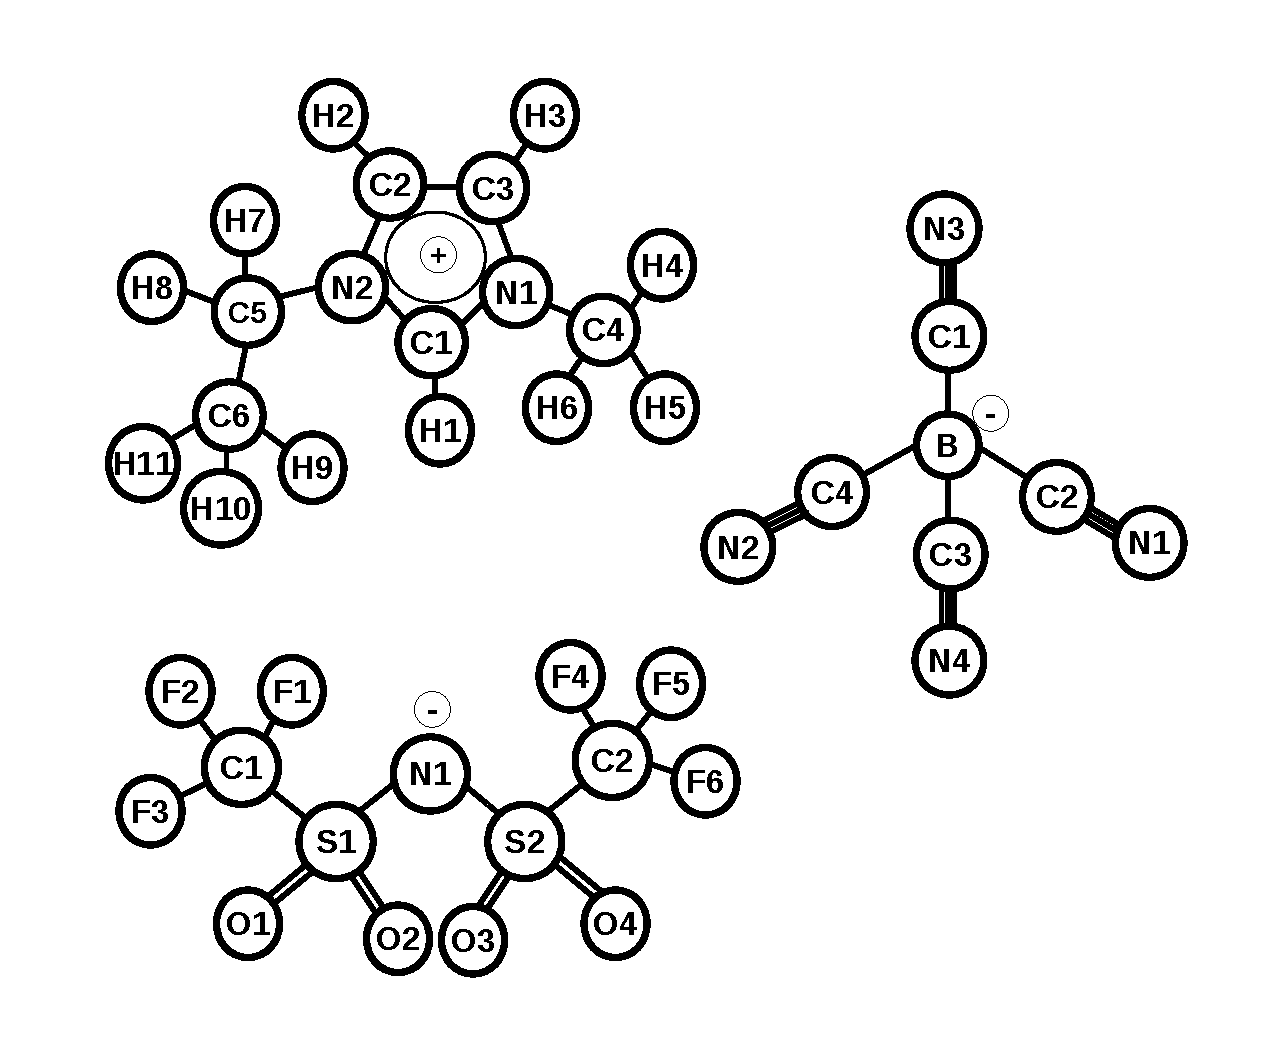
\includegraphics[width=\linewidth]{ions_paper.pdf}
\caption{[emim]$^{+}$ [B(CN)\textsubscript{4}]$^{-}$ [Tf\textsubscript{2}N]$^{-}$.}
\label{fig:scheme}
\end{figure}

rigid-body configurations: We first carried out simulations of the isolated ion pairs in order to obtain the minimum energy configurations with respect to the corresponding (classical) model for each case.

\begin{table*}[htp]
\caption{Densidades de [emim][B(CN)\textsubscript{4}] calculadas a partir simulaciones de NPT DM 298.15 K y 1 atm. La densidad experimental corresponde a $\rho^{\text{exp}}$ = 1.036 g/cm$^{3}$~\cite{Doma_ska_2011}.}
\begin{threeparttable}
\begin{tabular}{ c  c  c  c  c}  
\hline \hline
$\text{[emim]}$[B(CN)\textsubscript{4}] & $T_{\text{sim}}$ & $ P_{\text{sim}} $ & $\rho_{\text{sim}}$ & error (\%)\tnote{a} \\
model & (K) &  (atm) &  (g/cm$^{3}$) &  \\
			\hline
		 \multicolumn{5}{c}{Flexible ions/Ewald method}\\

Koller y col.~\cite{Koller_2012}  & 298.14 $\pm$  0.02 & 0 $\pm$ 2 & 1.046 & 1.0 \\
Batista y col.~\cite{Batista_2015} & 298.15 $\pm$ 0.01  & 1 $\pm$ 1 & 0.989 & 4.6  \\
Liu y col.~\cite{Liu_2014}  & 298.14 $\pm$ 0.01 & 0 $\pm$ 1 & 1.001 & 3.4  \\
Weber y Kirchner.~\cite{Weber_2016}  & 298.16  $\pm$ 0.01 & 1 $\pm$ 1 & 1.015 & 2.1  \\
	 \multicolumn{5}{c}{Rigid ions/DSF method}\\
Koller y col.~\cite{Koller_2012}   & 298.42  $\pm$ 0.03  & 1 $\pm$ 1 & 1.038 & 0.2 \\
Batista y col.~\cite{Batista_2015} & 298.43 $\pm$ 0.02  & 0.9 $\pm$ 0.7  & 0.988 & 4.7  \\
Liu y col.~\cite{Liu_2014}  & 298.46 $\pm$ 0.02 & 1.2  $\pm$ 0.8 & 0.991 &  4.4 \\
Weber y Kirchner.~\cite{Weber_2016} &  298.41 $\pm$ 0.03 & 1.1 $\pm$ 0.8 & 1.022 & 1.4  \\
 \hline \hline
\label{table:props_dsf} 
\end{tabular}
\begin{tablenotes}
\item[a] error = 100 $\times$($\rho^{\text{exp}}$$ - $$\rho^{\text{sim}}$)/$\rho^{\text{exp}}$.
\end{tablenotes}
\end{threeparttable}
\end{table*}


\begin{figure*}
\centering
\subfloat[text for the first subfigure\label{sfig:testa}]{%
  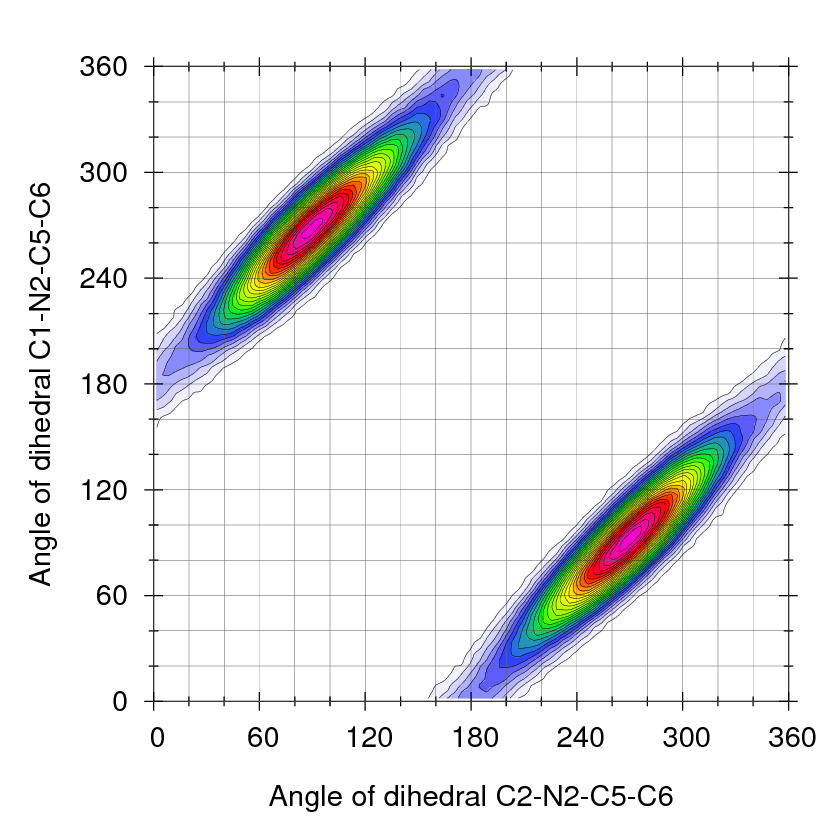
\includegraphics[width=.4\linewidth]{koller}%
}
\subfloat[text for the second subfigure\label{sfig:testa}]{%
  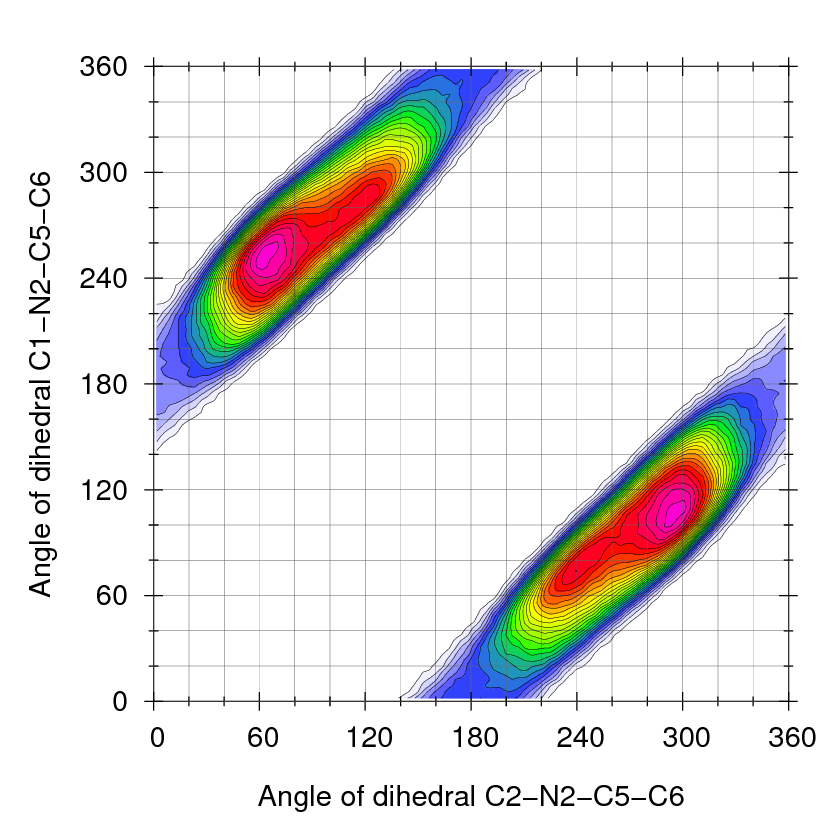
\includegraphics[width=.4\linewidth]{batista}%
}

\subfloat[text for the second subfigure\label{sfig:testa}]{%
  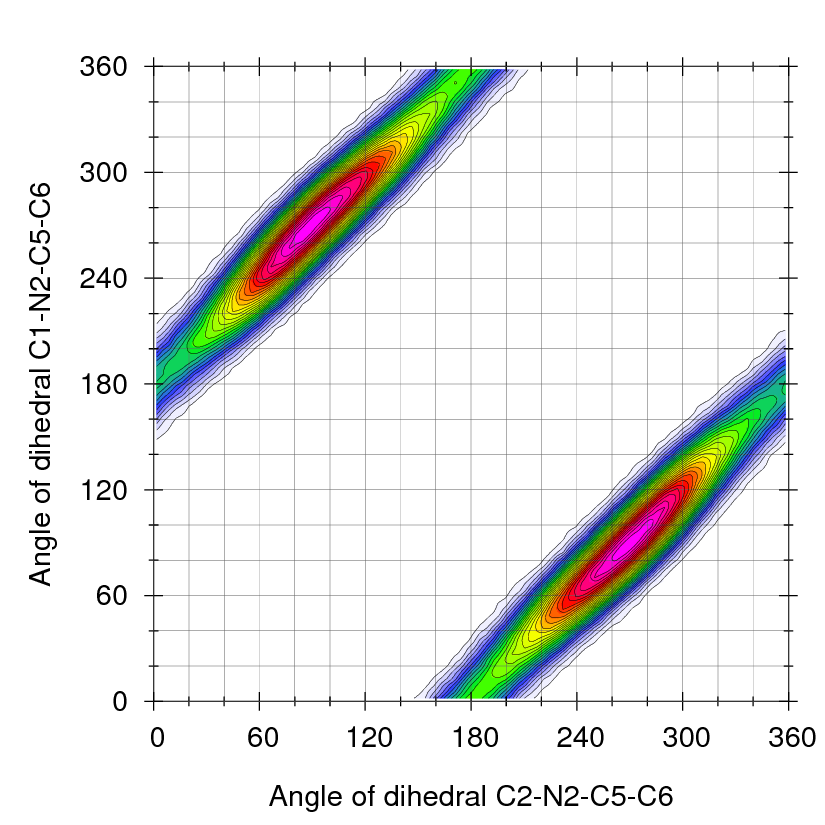
\includegraphics[width=.4\linewidth]{Liu}%
}
\subfloat[text for the second subfigure\label{sfig:testa}]{%
  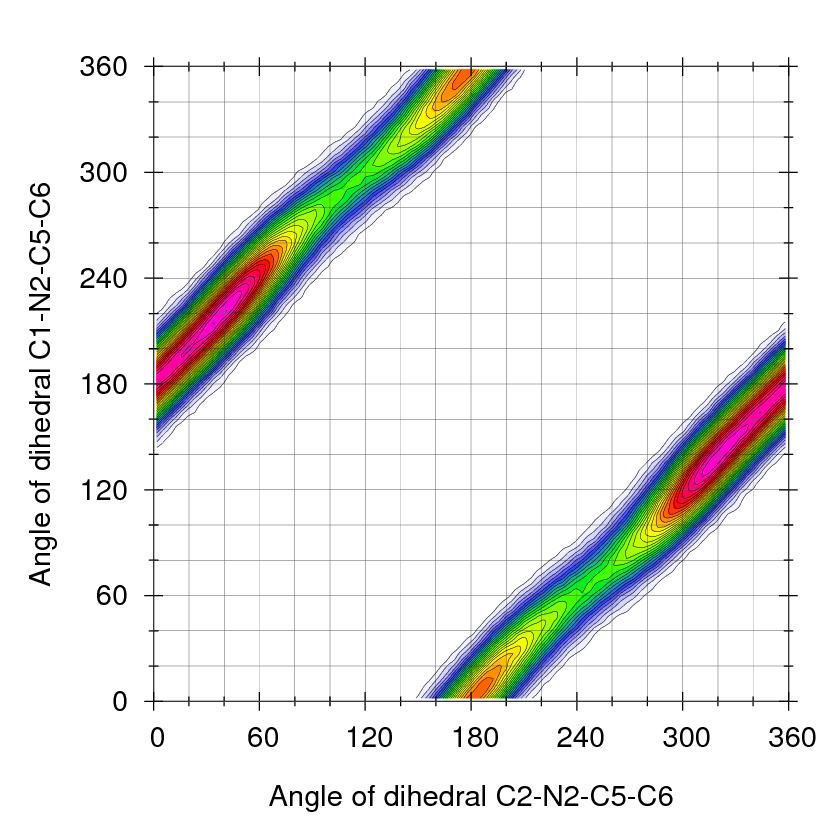
\includegraphics[width=.4\linewidth]{Weber}%
}
\caption{}
\label{}
\end{figure*}


\begin{figure}
\centering
\subfloat[text for the first subfigure\label{sfig:testa}]{%
  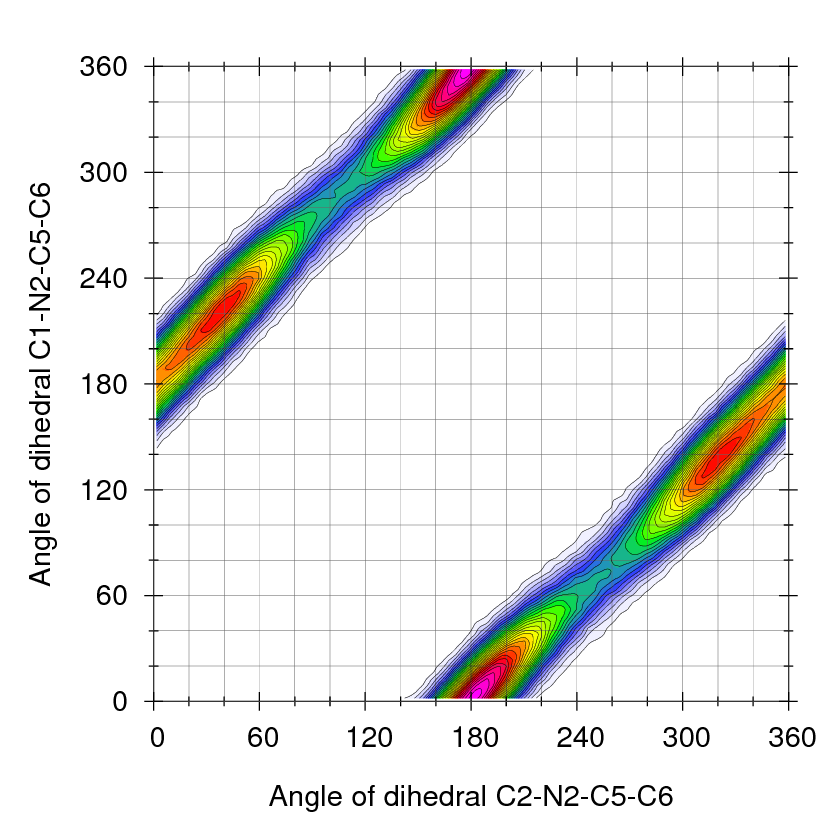
\includegraphics[width=\linewidth]{Ludwig}%
}

\subfloat[text for the second subfigure\label{sfig:testa}]{%
  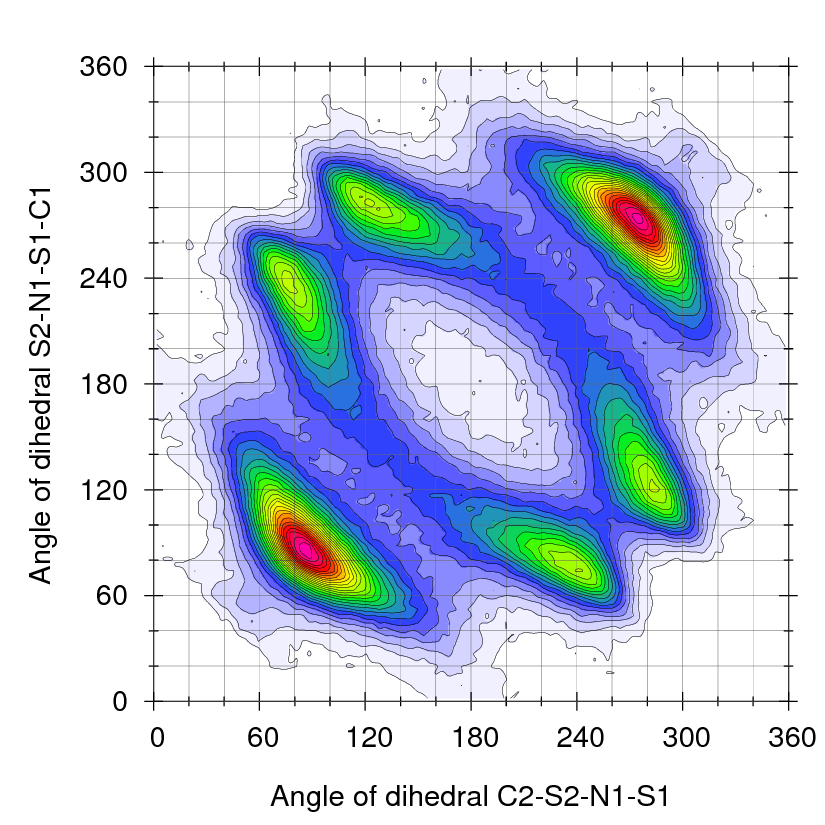
\includegraphics[width=\linewidth]{Ludwig_anion}%
}
\caption{}
\label{}
\end{figure}

\subsection{Henry constant of CO\textsubscript{2} in [emim][B(CN)\textsubscript{4}] and [emim][Tf\textsubscript{2}N]}
\label{sec:henry_results}

\begin{table*}[htp]
\centering
\begin{adjustbox}{width=1\textwidth}
\begin{threeparttable}
\caption{Resultados de la energía libre de solvatación y de la constante de Henry de CO\textsubscript{2} en [emim][B(CN)\textsubscript{4}] y [emim][Tf\textsubscript{2}N] a T = 298.15 K y P = 1 atm. Los valores experimentales de la constante de Henry en [emim][B(CN)\textsubscript{4}] y [emim][Tf\textsubscript{2}N] corresponden a 38.9 $\pm$ 0.03 atm~\cite{Mahurin_2010} y a 39.0 $\pm$ 0.1 atm~\cite{Finotello_2008}, respectivamente.}
\begin{tabular}{ c c c  c  c  c  c }  
\toprule
Modelo & $\tilde{\rho}_{\text{sim}}$ & $\Delta G_{\,\text{LJ}}$  & $\Delta G_{\,\text{Coul}}$  & $\Delta G_{\,\text{sim}}$ & $K_{s}$ & error (\%)\tnote{a}\\
& (mol/dm$^{3}$) & (kcal/mol) & (kcal/mol) &  (kcal/mol) & (atm)  &  \\
			\hline
			\multicolumn{4}{c}{[emim][B(CN)\textsubscript{4}]} & \multicolumn{2}{c}{\cellcolor{gray!25}$K_{s}^{\text{exp}}$ = 38.9 $\pm$ 0.03 atm~\cite{Mahurin_2010}}\\
			\hline
Koller y col.~\cite{Koller_2012} & 4.5925 & 0.45 $\pm$ 0.01 & -1.06 $\pm$ 0.02 & -0.61 $\pm$ 0.02 & 40 $\pm$ 1 & 2.8 \\
Batista y col.~\cite{Batista_2015} & 4.3700 & 0.378 $\pm$ 0.008 & -1.24 $\pm$ 0.01  & -0.86 $\pm$ 0.01 & 24.9 $\pm$ 0.5 & 38.9 \\
Liu y col.~\cite{Liu_2014} & 4.3815 & 0.226 $\pm$ 0.009 & -1.11 $\pm$ 0.01 & -0.88 $\pm$ 0.01 & 24.3 $\pm$ 0.5 & 37.6  \\
Weber y Kirchner~\cite{Weber_2016} & 4.5221 & 0.478 $\pm$ 0.009 & -1.23 $\pm$ 0.02 & -0.75 $\pm$ 0.02 & 31 $\pm$ 1 & 20.3  \\
\hline
		\multicolumn{4}{c}{[emim][Tf\textsubscript{2}N]} & \multicolumn{2}{c}{ \cellcolor{gray!25} $K_{s}^{\text{exp}}$ = 39.0 $\pm$ 0.1 atm~\cite{Finotello_2008}}\\
		\hline
 K\"{o}ddermann y col.~\cite{K_ddermann_2007} &3.8205 & 0.389 $\pm$ 0.005 & -0.901 $\pm$ 0.006& -0.512 $\pm$ 0.008 & 39.4 $\pm$ 0.5  & 0.97  \\
 \bottomrule
\label{table:henry} 
\end{tabular}
\begin{tablenotes}
\item[a] error = 100 $\times$ $\abs{(K_s^{\text{exp}} - K_s^{\text{sim}})/K_s^{\text{exp}}}$.
\end{tablenotes}
\end{threeparttable}
\end{adjustbox}
\end{table*}

\begin{figure}
\centering
\subfloat[text for the first subfigure\label{sfig:testa}]{%
  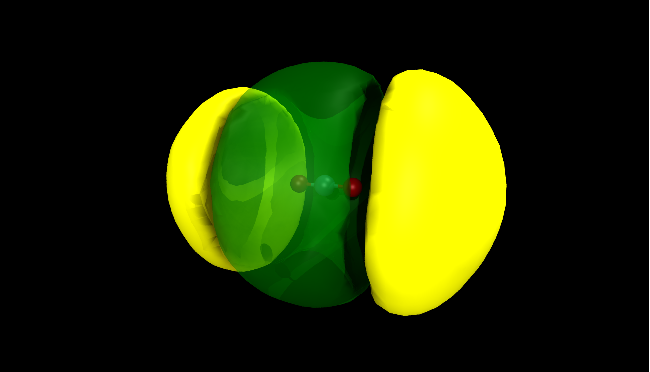
\includegraphics[width=\linewidth]{kollerall.pdf}%
}

\subfloat[text for the second subfigure\label{sfig:testa}]{%
  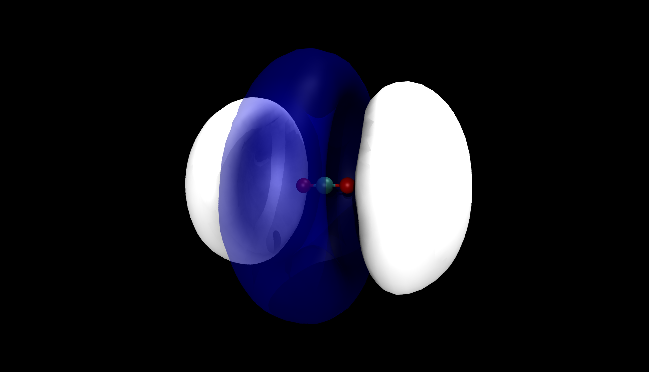
\includegraphics[width=\linewidth]{ludwigall.pdf}%
}
\caption{}
\label{}
\end{figure}

\subsection{Inifinite-dilution activity coefficient in [emim] [B(CN)\textsubscript{4}]}
\label{sec:act_results}

\begin{table*}[htp]
\centering
\begin{adjustbox}{width=1\textwidth}
\begin{threeparttable}
\caption{Resultados de la energía libre de solvatación a T = 298.15 K de las sustancias puras benceno, hexano, ciclohexano, etanol y agua.}
\begin{tabular}{ c c c c c c c c }
\toprule
Soluto & $\rho_{\text{sim}}$ & error (\%)\tnote{a} & $\Delta G_{\,\text{LJ}}$  & $\Delta G_{\,\text{Coul}}$  & $\Delta G^{0}_{\,\text{sim}}$ & $\Delta G^{\text{0,exp}}$   & error (\%)\tnote{a}\\
 & (g/cm$^{3}$) &  & (kcal/mol) &  (kcal/mol) &  (kcal/mol)   &  \\
\hline
benceno OPLS-AA   & 0.8611 $\pm$ 0.0002 & 1.4 & -3.75  $\pm$ 0.02 & -0.381 $\pm$ 0.007 & -4.14 $\pm$ 0.02 & -4.56 & 9.32  \\
hexano OPLS-AA    & 0.6513 $\pm$ 0.0003 & 0.5 & -3.67  $\pm$  0.03 & 0.011 $\pm$ 0 & -3.66 $\pm$ 0.03 & -4.06 & 9.90 \\
ciclohexano & 0.7692 $\pm$ 0.0007 & 0.6 & -4.39 $\pm$ 0.01 & 0 & -4.39 $\pm$ 0.01 & - & -  \\
etanol TRAPPE-UA   & 0.781 $\pm$ 0.008 & 1.01  &-0.93 $\pm$ 0.01 & -4.15 $\pm$ 0.02  & -5.08  $\pm$ 0.02  & -5.08 & 0 \\
agua TIP4P/2005   &  0.9948 $\pm$ 0.0003 & 0.2 & 2.015 $\pm$ 0.004 & -9.01 $\pm$ 0.02 & -6.99 $\pm$ 0.02 & -6.33  &10.43 \\
 \bottomrule
\label{table:mu_solutos} 
\end{tabular}
\begin{tablenotes}
\item[a] error = 100 $\times$ $\abs{(Z^{\text{exp}} - Z^{\text{sim}})/Z^{\text{exp}}}$.
\end{tablenotes}
\end{threeparttable}
\end{adjustbox}
\end{table*}

\begin{table*}[htp]
\centering
\begin{adjustbox}{width=1\textwidth}
\begin{threeparttable}
\caption{Coeficientes de actividad a dilución infinita en [emim][B(CN)\textsubscript{4}] a T = 298.15 K de los solutos benceno, hexano, ciclohexano, etanol y agua.}
\begin{tabular}{c c c c c c  >{\columncolor[gray]{0.8}} c}  
\toprule
Soluto & $\Delta G_{\,\text{LJ}}$  & $\Delta G_{\,\text{Coul}}$  & $\Delta G_{\,\text{sim}}$  & $\gamma^{\,\infty,\text{sim}}$ & $\gamma^{\, \infty,\text{exp}}$ & $\gamma^{\, \infty,\text{exp}}$  \\
 & (kcal/mol) & (kcal/mol) &  (kcal/mol)  &  & (298.15 K) \cite{Doma_ska_2011} & (303 K) \cite{Yan_2010} \\
\midrule % inserts single-line
hexano OPLS-AA & -2.13 $\pm$ 0.04 & -0.152 $\pm$ 0.007 & -2.282 $\pm$ 0.04 & 6.2 $\pm$ 0.5 & 33.8 & 20.97  \\
ciclohexano& -2.75 $\pm$ 0.06 & - & -2.75 $\pm$ 0.06 & 9 $\pm$ 1 & 16.7 & 13.82 \\
benceno OPLS-AA  & -2.23 $\pm$ 0.05 & -1.29 $\pm$ 0.04 & -3.52 $\pm$ 0.06 & 1.2 $\pm$ 0.1 & 1.13 & 1.31 \\ 
ethanol TRAPPE-UA& -0.73 $\pm$ 0.02 & -4.10 $\pm$ 0.04 & -4.83 $\pm$ 0.04 & 0.41 $\pm$ 0.03 & 1.58 & 1.64  \\
agua TIP4P/2005& 1.38 $\pm$ 0.008 & -6.32 $\pm$ 0.03 & -4.94 $\pm$ 0.03 & 2 $\pm$ 1 & 2.65 & 2.24 \\
 \bottomrule
\label{table:gamma} 
\end{tabular}
\end{threeparttable}
\end{adjustbox}
\end{table*}

\subsection{Study of concentrated solutions of CO\textsubscript{2} in [emim][B(CN)\textsubscript{4}] and [emim][Tf\textsubscript{2}N]}
\label{sec:prel_results}

\section{Concluding remarks}
\label{sec:conclusion}

\section*{Acknowledgments}
The authors acknowledge the financial support provided by Petrobras (project code CENPES 16113). 

\section*{References}

\bibliography{mybibfile}
%\begin{equation}
%\begin{split}
%\Delta G_{\text{sim}} - k_b T \ln \left( \frac{V^{\ast}}{V_1} \right) &= k_b T \ln \left(\frac{P_s}{x_s} \frac{1}{\tilde{\rho}_{\scaleto{LI}{4pt}}} \right) \\
%&= k_b T \ln \left( \frac{K_s}{\tilde{\rho}_{\scaleto{LI}{4pt}} R T} \right),
%\end{split}
%\end{equation}
\end{document}